\documentclass[plain,basic]{inVerba-notes}

\newcommand{\userName}{Cullyn Newman}
\newcommand{\class}{BI:\@ 428}
\newcommand{\theTitle}{Journal Article Summary --- Week 6}
\newcommand{\institution}{Portland State University}
%chktex-file 8
\begin{document}    

\begin{center}
    \textbf{\Large{The role of exome sequencing in newborn screening for inborn errors of metabolism}}
\end{center}

\section{Key Points}
\begin{itemize}
    \item \textbf{Newborn Screening (NBS)}: public health newborn screening that on a population scale aimed to identify rare, treatable conditions in infants.
    \item \textbf{Tandem Mass Spectrometry (MS/MS)}: a technique where two or more mass spectrometry tests are coupled together with an additional reaction step to increase their analytical ability, specifically in rare inborn errors in this study's case.
    \item \textbf{Inborn Errors of Metabolism (IEMs)}: a class of genetic diseases that involve birth defects and disorders of metabolism; generally do errors in enzyme coding genes.
    \item \textbf{Whole Exome Sequencing (WES)}: a genomic technique for sequencing all the protein-coding regions of genes in the genome (i.e., the exome). 
    \item WES was used as an innovative methodology for NBS\@;
        \begin{itemize}
            \item This study used archived blood data from nearly all  infants with IEMs in the 4.35 million born from 2005 to 2013, including those with false positive MS/MS tests.
            \item WES had overall sensitivity of 88\% and specificity of 98.4\%.        
            \item MS/MS had 99.0\% and 99.8\% respectively.
            \item WES could be used as secondary test for false positive screening of MS/MS tests.
        \end{itemize}
    \item This study represents the largest sequencing effort of an entire population study of IEM-affected cases to date, allowing for unbiased assessment of WES as tool for population screening.
\end{itemize}

\section{Background}
\begin{itemize}
    \item Genomic sequencing is recommended and used for diagnoses of rare disorders, with a strong recommendation for children intensive care units, however population studies are underreported. 
    \item NBS IEMs useful for identifying well studied Mendelian disorders.
    \item WES used to identify IEMs already included in NBS suggests potential utility for disorders missed by MS/MS\@.
    \item This study used an automated pipeline with three separate arms to investigate various parameters in order to create a means for reporting disease-causing variants in IEM genes with in screening contexts.
\end{itemize}

\clearpage 
\section{Figures Used in Discussion}

\begin{center}
    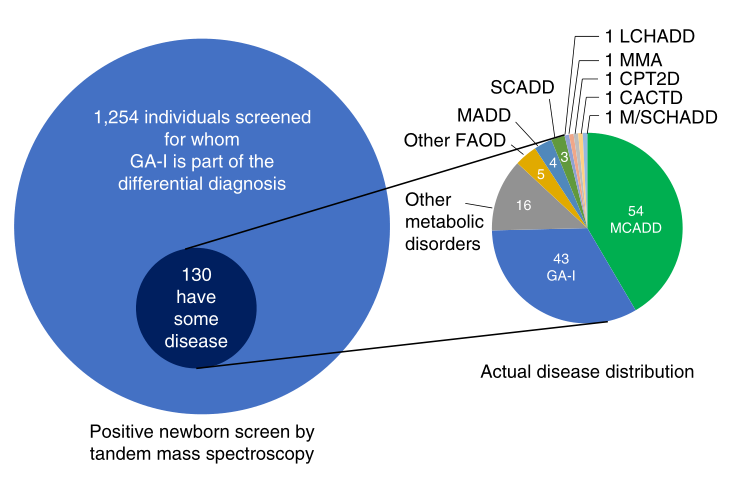
\includegraphics[scale=0.44]{images/fig-6-1.png} 
    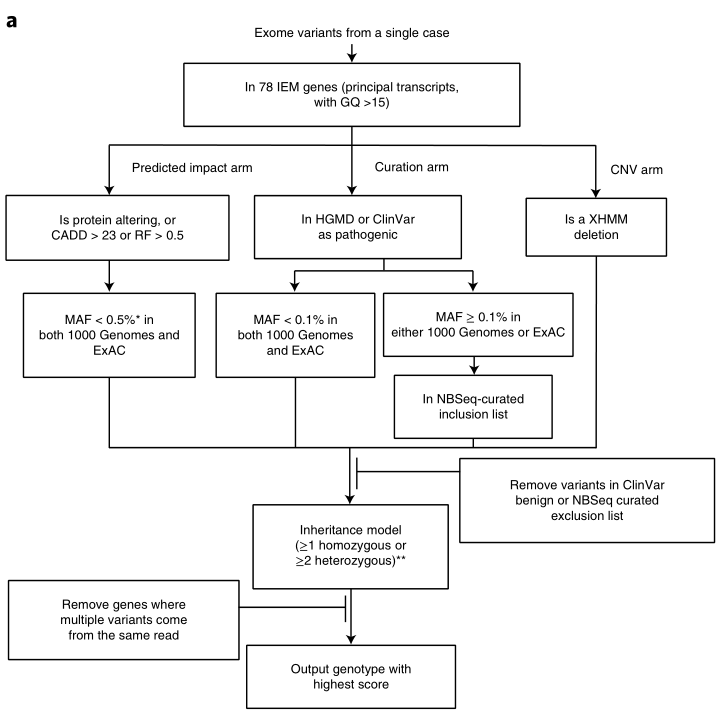
\includegraphics[scale=0.63]{images/fig-6-2a.png} 
\end{center}

\nocite{adhikari2020role}
\bibliographystyle{apacite}
\bibliography{summaries.bib}
\end{document}

